% Tamaño del papel
% ISO A series:
% a0	ISO A0 paper size (83.96cm × 118.82cm); normal font size 25pt.
% a1	ISO A1 paper size (59.4cm × 83.96cm); normal font size 20pt.
% a2	ISO A2 paper size (41.98cm × 59.4cm); normal font size 17pt.
% a3	ISO A3 paper size (29.7cm × 41.98cm); normal font size 14pt.
% ANSI Sizes:
% ansiE	ANSI E paper size (86.36cm × 111.76cm); normal font size 25pt.
% ansiD	ANSI D paper size (55.88cm × 86.36cm); normal font size 20pt.
% ansiC	ANSI C paper size (43.18cm × 55.88cm); normal font size 17pt. tabloid 
%	Tabloid, a.k.a. ledger, a.k.a. ANSI B paper size (27.9cm × 43.18cm); normal font size 14pt.
% Para formato vertical hay que quitar la opción landscape

%\documentclass[a2, landscape]{sciposter}
% poster de tamaño a2, en horizontal,sombra para los titulos
%\documentclass[a2, landscape, plainboxedsections]{sciposter}
\documentclass[a2,plainboxedsections]{sciposter}

\usepackage{amsmath, amssymb, latexsym}
\usepackage[utf8]{inputenc}
\usepackage{graphicx}
\usepackage{multicol}
\usepackage[spanish, mexico]{babel}

% Color fondo cabecera de sección 
%\definecolor{BoxCol}{cmyk}{0.8,0.52,0,0.67}
\definecolor{BoxCol}{rgb}{0.17,0.16,0.27}

% Color fuente cabecera de sección
\definecolor{SectionCol}{cmyk}{0,0,0,0}
%\definecolor{SectionCol}{rgb}{0.9,0.86,0.85}

\leftlogo[1]{Escudo-UNAM}
\rightlogo[1]{Escudo-FC}

%\noleftlogo
%\norightlogo
%\nologos

\usepackage{color}

%\title{Elipse}
\title{\color{blue}{Elipse}}
\author{Juan M. Barrios}
\institute{CSC, Facultad de Ciencias\\
	Universidad Nacional Autónoma de México\\}
%	México}
\email{j...@ciencias.unam.mx}
%Nombre de la conferencia a la que se asistio
\conference{\textbf{CL 2013}, Curso de introduccón a \LaTeX{}, junio de 2014}

\begin{document}
\maketitle

% Si el poster esta en modo landscape (horizontal) usar 5 columnas en otro caso usar 3
\begin{multicols}{3}
%\begin{multicols}{5}

\section{Historia}

\color{magenta} \PARstart{F}{orma} elíptica trazada en la antigüedad sobre un muro de Tebas (Egipto). \color{black}
Forma elíptica trazada en la antigüedad sobre un muro de Tebas (Egipto).
La elipse, como curva geométrica, fue estudiada por Menecmo, investigada por Euclides, y su nombre se atribuye a Apolonio de Perge. El foco y la directriz de la sección cónica de una elipse fueron estudiadas por Pappus. En 1602, Kepler creía que la órbita de Marte era ovalada, aunque más tarde descubrió que se trataba de una elipse con el Sol en un foco. De hecho, Kepler introdujo la palabra «focus» y publicó su descubrimiento en 1609. Halley, en 1705, demostró que el cometa que ahora lleva su nombre trazaba una órbita elíptica alrededor del Sol.

\section{Elementos de una elipse}
La elipse es una curva plana y cerrada, simétrica respecto a dos ejes perpendiculares entre sí:
\begin{itemize}
	\item El semieje mayor (el segmento C-a de la figura), y
	\item el semieje menor (el segmento C-b de la figura).
\end{itemize}
Miden la mitad del eje mayor y menor respectivamente.

\begin{figure}
	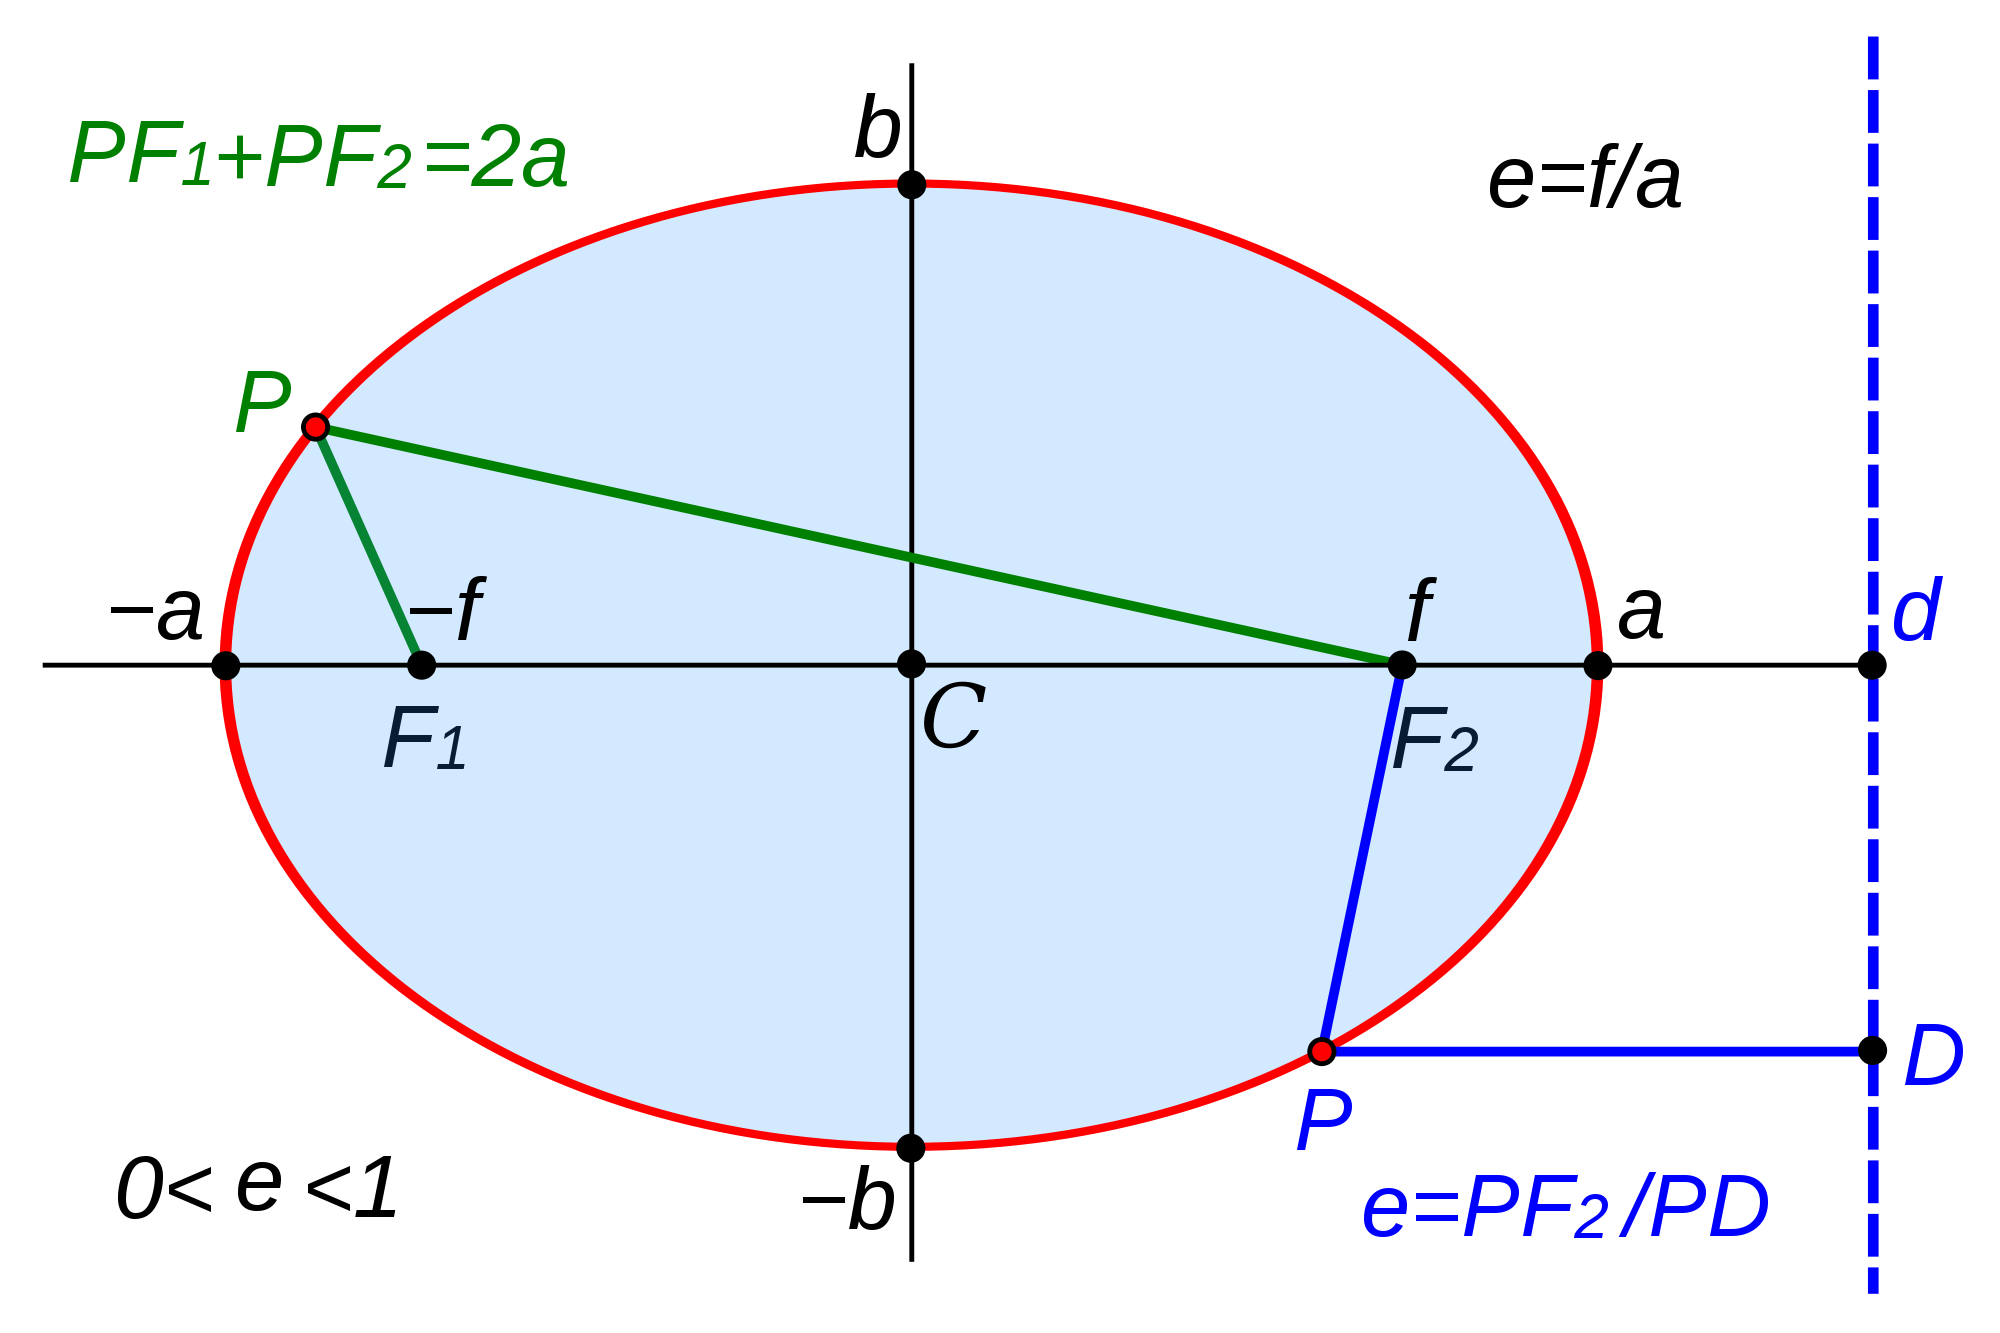
\includegraphics[width=\textwidth]{elipse1}
\end{figure}

\subsection{Puntos de una elipse}

Los focos de la elipse son dos puntos equidistantes del centro, $F_1$ y $F_2$ en el eje mayor. La suma de las distancias desde cualquier punto $P$ de la elipse a los dos focos es constante, e igual a la longitud del diámetro mayor, ($PF_1 + PF_2 = 2a$).

Si $F_1$ y $F_2$ son dos puntos de un plano, y $2a$ es una constante mayor que la distancia $F_1F_2$, un punto $P$ pertenecerá a la elipse si se cumple la relación:
\[
P F_1 + P F_2 = 2a 
\]
donde $a$ es la medida del semieje mayor de la elipse.

\subsection{Ejes de una elipse}

El eje mayor $2a$, es la mayor distancia entre dos puntos adversos de la elipse. El resultado constante de la suma de las distancias de cualquier punto a los focos equivale al eje mayor. El eje menor $2b$, es la menor distancia entre dos puntos adversos de la elipse. Los ejes de la elipse son perpendiculares entre si.

\subsection{Excentricidad de una elipse}

La excentricidad $\epsilon$ (épsilon) de una elipse es la razón entre su semidistancia focal (segmento que va del centro de la elipse a uno de sus focos), denominada por la letra $c$, y su semieje mayor. Su valor se encuentra entre cero y uno.

\[
\epsilon=\frac{c}{a},\mbox{ con }0\leq\epsilon\leq1
\]
Dado que $c = \sqrt{a^2-b^2}$, también vale la relación:
\[
\epsilon=\sqrt{\frac{a^2-b^2}{a^2}}
    =\sqrt{1-\left(\frac{b}{a}\right)^2}
 \]
o el sistema:
\[
\begin{cases}
\epsilon=\frac{c}{a}\\
c = \sqrt{a^2-b^2} \end{cases}
\]

La excentricidad indica la forma de una elipse; una elipse será más redondeada cuanto más se aproxime su excentricidad al valor cero. La designación tradicional de la excentricidad es la letra griega $\epsilon$ llamada épsilon.

(No se debe usar la letra $e$ para designarla, porque se reserva para la base de los logaritmos naturales o neperianos.).

\subsection{Excentricidad angular de una elipse}

La excentricidad angular $\alpha$ es el ángulo para el cual el valor de la función trigonométrica seno concuerda con la excentricidad $\epsilon$, esto es:
\begin{align*}
\alpha&=\sin^{-1}(\epsilon)=\cos^{-1}\left(\frac{b}{a}\right)\\
&=2\tan^{-1}\left(\sqrt{\frac{a-b}{a+b}}\right);
\end{align*}

\subsection{Constante de la elipse}

Como establece la definición inicial de la elipse como lugar geométrico, para todos los puntos $P$ de la elipse la suma de las longitudes de sus dos radio vectores es una cantidad constante igual a la longitud $2a$ del eje mayor:
\[
PF_1 + PF_2 = 2a
\]

\subsection{Directrices de la elipse}

\begin{figure}
 	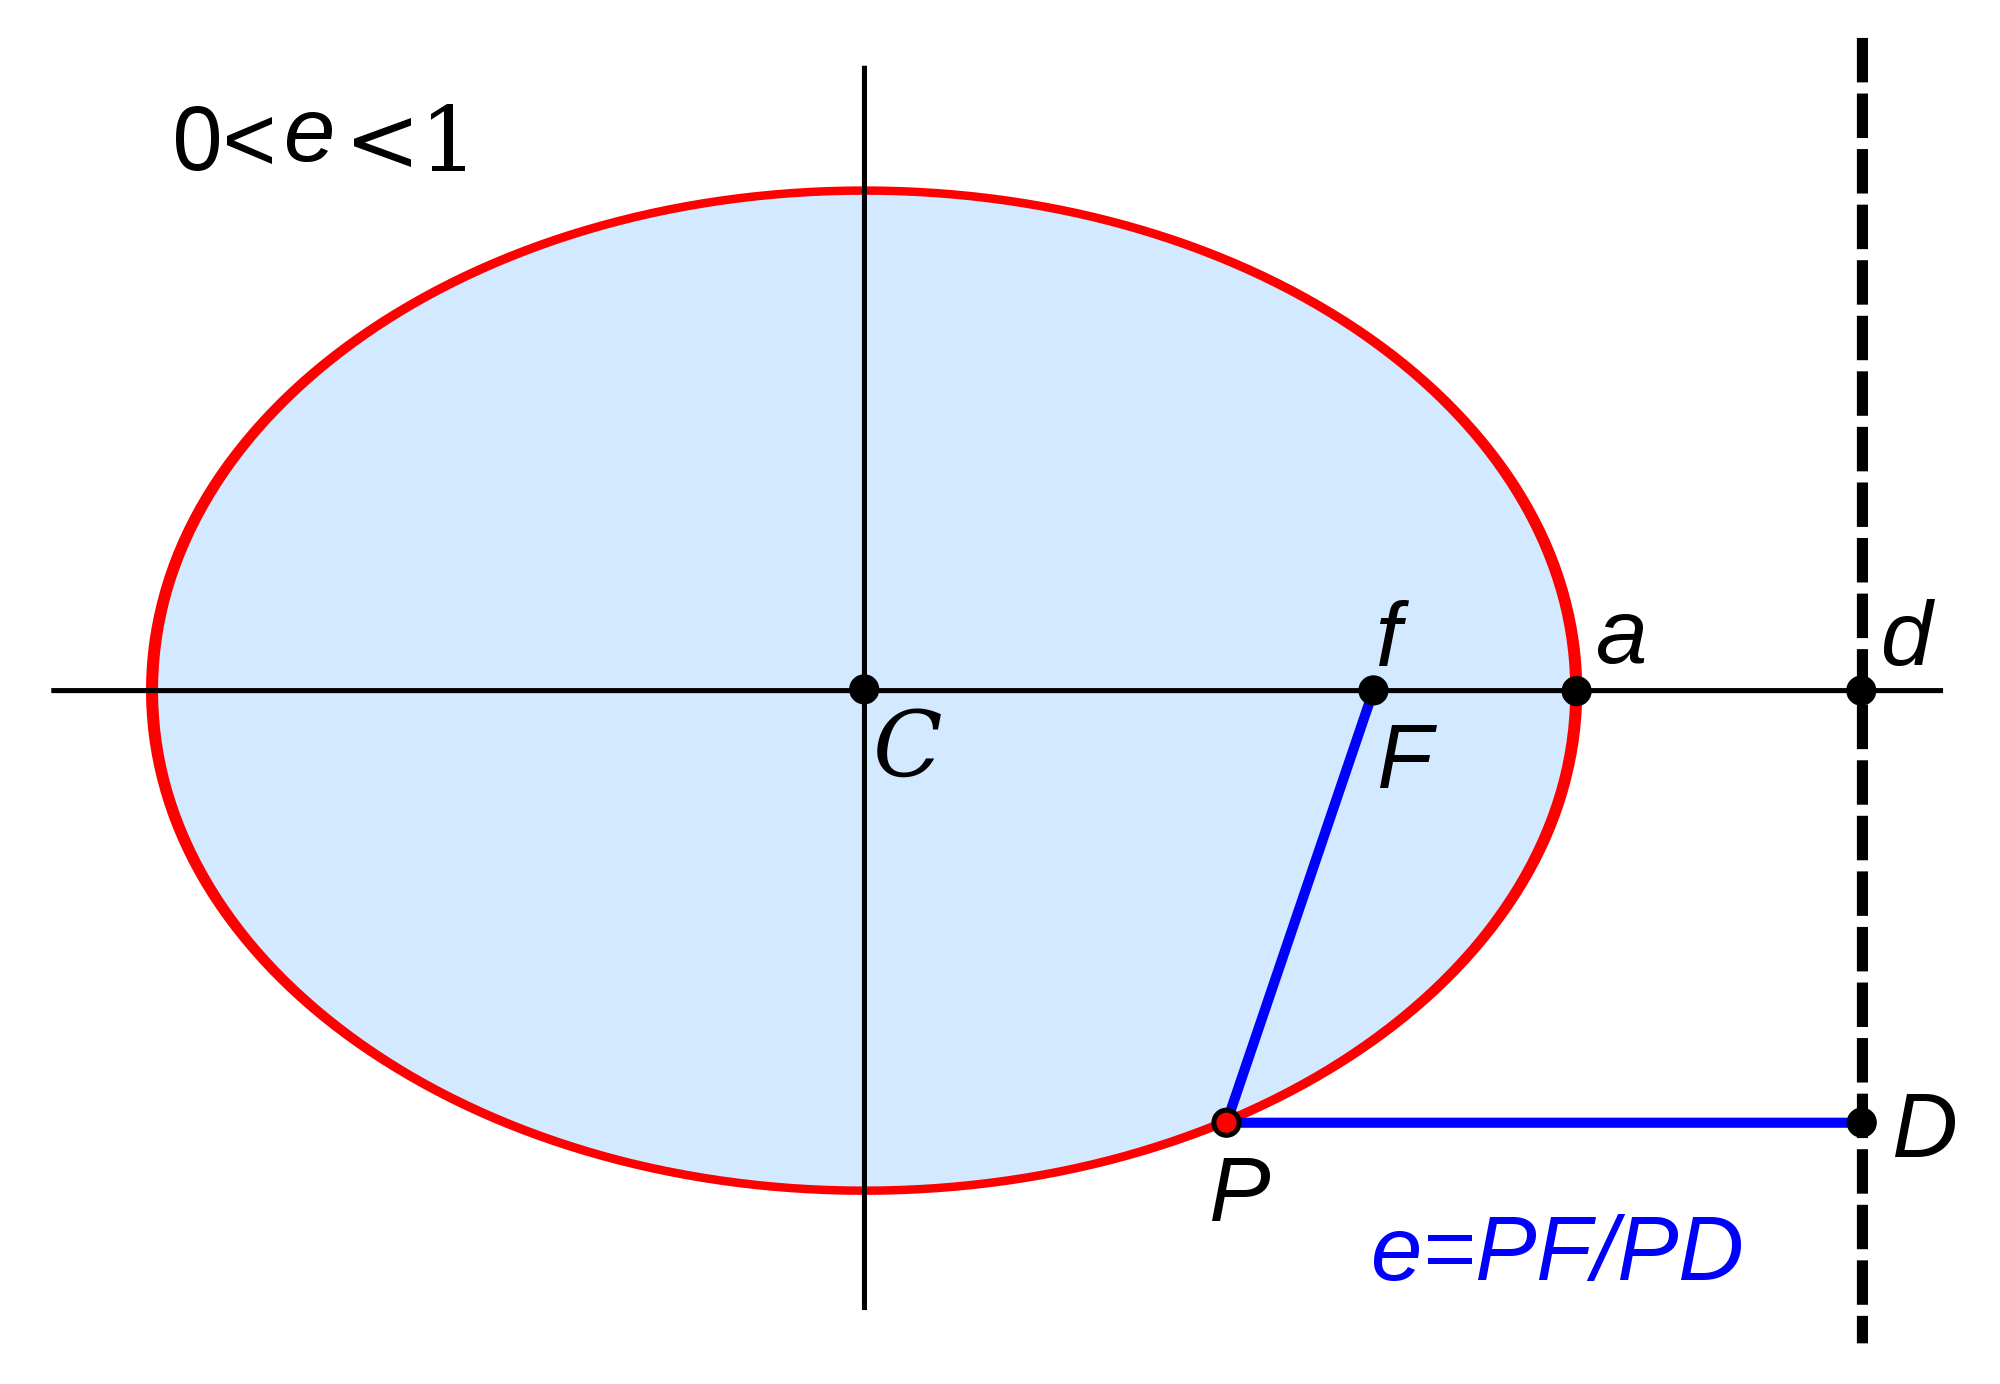
\includegraphics[width=\textwidth]{elipse2}
	\caption{La recta $dD$ es una de las 2 directrices de la elipse.}\label{figura2}
\end{figure}

Cada foco $F$ de la elipse está asociado con una recta paralela al semieje menor llamada directriz (ver figura~\ref{figura2}). La distancia de cualquier punto $P$ de la elipse hasta el foco $F$ es una fracción constante de la distancia perpendicular de ese punto $P$ a la directriz que resulta en la igualdad:
\[
\epsilon=\frac{\overline{\text{PF}}}{\overline{\text{PD}}}
\]
La relación entre estas dos distancias es la excentricidad $\epsilon$ de la elipse. Esta propiedad (que puede ser probada con la herramienta esferas de Dandelin) puede ser tomada como otra definición alternativa de la elipse.

Una elipse es el lugar geométrico de todos los puntos de un plano para los cuales se cumple que el cociente entre sus distancias a un punto fijo –que se denomina foco– y a una recta dada –llamada directriz– permanece constante y es igual a la excentricidad de la misma.

Además de la bien conocida relación $\epsilon=\frac{f}{a}$, también es cierto que $\epsilon=\frac{a}{d}$, también es útil la fórmula $d=\frac{a}{\epsilon}$.

Aunque en la figura solo se dibujó la directriz del foco derecho, existe otra directriz para el foco izquierdo cuya distancia del centro $O$ es $-d$, la cual además es paralela a la directriz anterior.
\end{multicols}
\end{document}